\begin{figure}[h]
	\centering
	\setlength{\resLen}{1.2in}
	\addtolength{\tabcolsep}{-3.5pt}
	\begin{tabular}{ccc}
		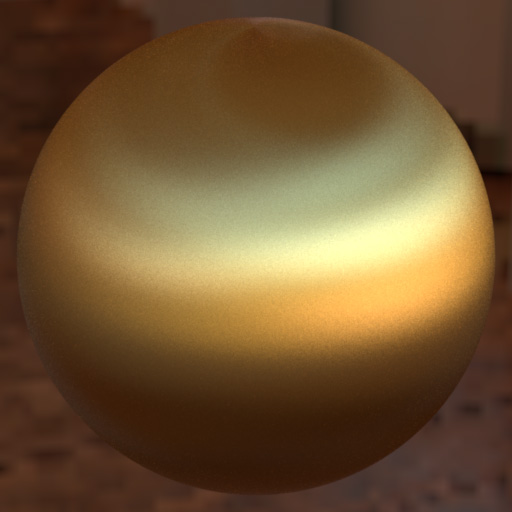
\includegraphics[width=\resLen]{layeredbsdf/validations/compare2/aniso_comb_hor_hor_512spp_17min.jpg} &
		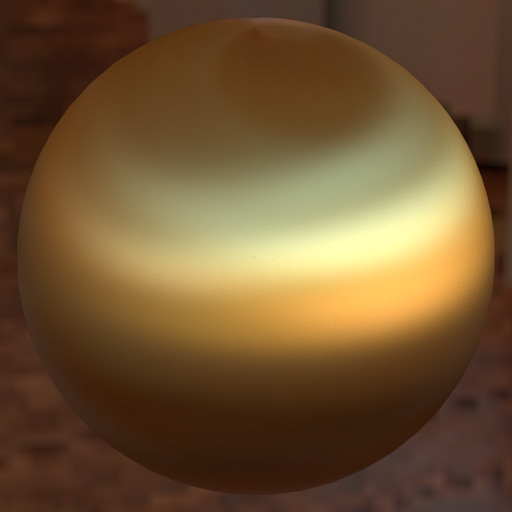
\includegraphics[width=\resLen]{layeredbsdf/validations/compare2/aniso_comb_hor_hor_wenzel.jpg} &
		
\includegraphics[width=\resLen]{layeredbsdf/validations/compare2/na.pdf} \\		
		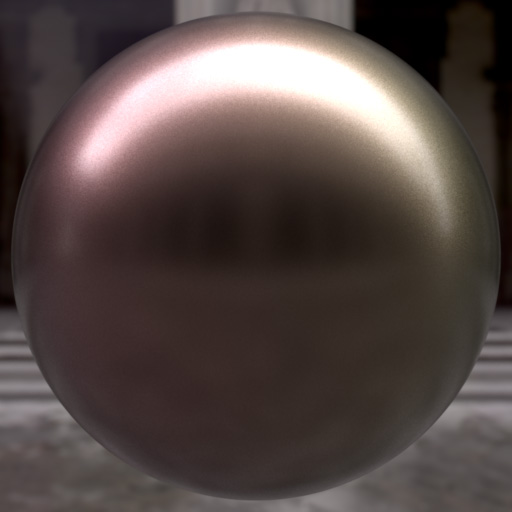
\includegraphics[width=\resLen]{layeredbsdf/validations/compare2/sphere_layered_1024spp_37min.jpg} &
		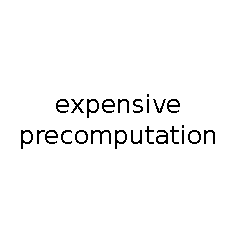
\includegraphics[width=\resLen]{layeredbsdf/validations/compare2/na2.pdf} &
		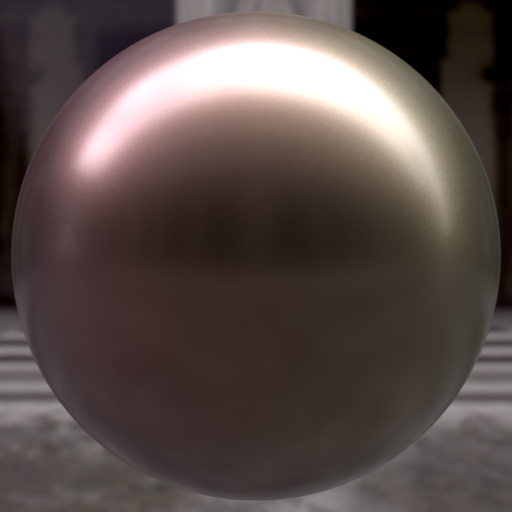
\includegraphics[width=\resLen]{layeredbsdf/validations/compare2/sphere_laurent_1024spp_1_5min.jpg} \\	
		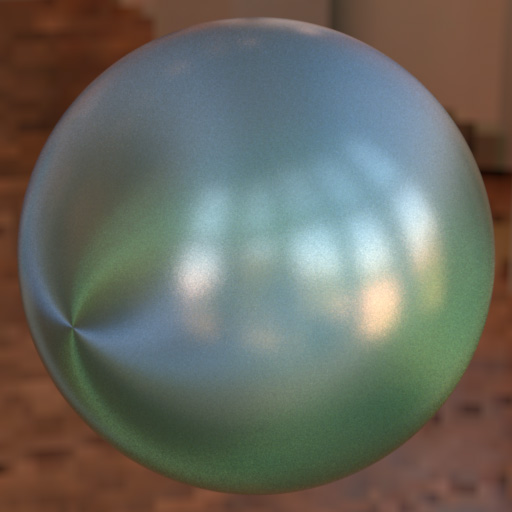
\includegraphics[width=\resLen]{layeredbsdf/validations/compare2/sphere_1024spp_60min.jpg} &
		
\includegraphics[width=\resLen]{layeredbsdf/validations/compare2/na.pdf} &
		
\includegraphics[width=\resLen]{layeredbsdf/validations/compare2/na.pdf} \\
		Ours &
		Zeltner 2018 \cite{zeltner2018layer} &
		Belcour 2018 \cite{belcour2018efficient}
	\end{tabular}
	\caption[Comparison to previous work]{\label{fig:layeredbsdf:compare_previous}
		\textbf{Comparison to previous work.} The \textbf{top row} shows an example with anisotropic surface reflectance, where our solution closely matches Zeltner's, but Belcour's approach does not support anisotropy. The \textbf{middle row} shows an example with spatial variation in the parameters; here our method closely matches Belcour's, but Zeltner's approach does not naturally support spatial variation. The \textbf{bottom row} shows a two-layer configuration with anisotropic microflake phase functions, which is only supported by our method.
	}
\end{figure}
